\chapter{CRAFTS Data Pipeline}
\label{ch:datapipe}
The goal of the CRAFTS data pipeline design is to be as modular as possible. We take a page from the Unix philosophy, every component of CRAFTS is designed to do one thing, do it well, and be easily swappable with alternate modules. A graphical representation of the CRAFTS data pipeline can be seen in \Cref{fig:workflow}.

\begin{figure}
    \centering
      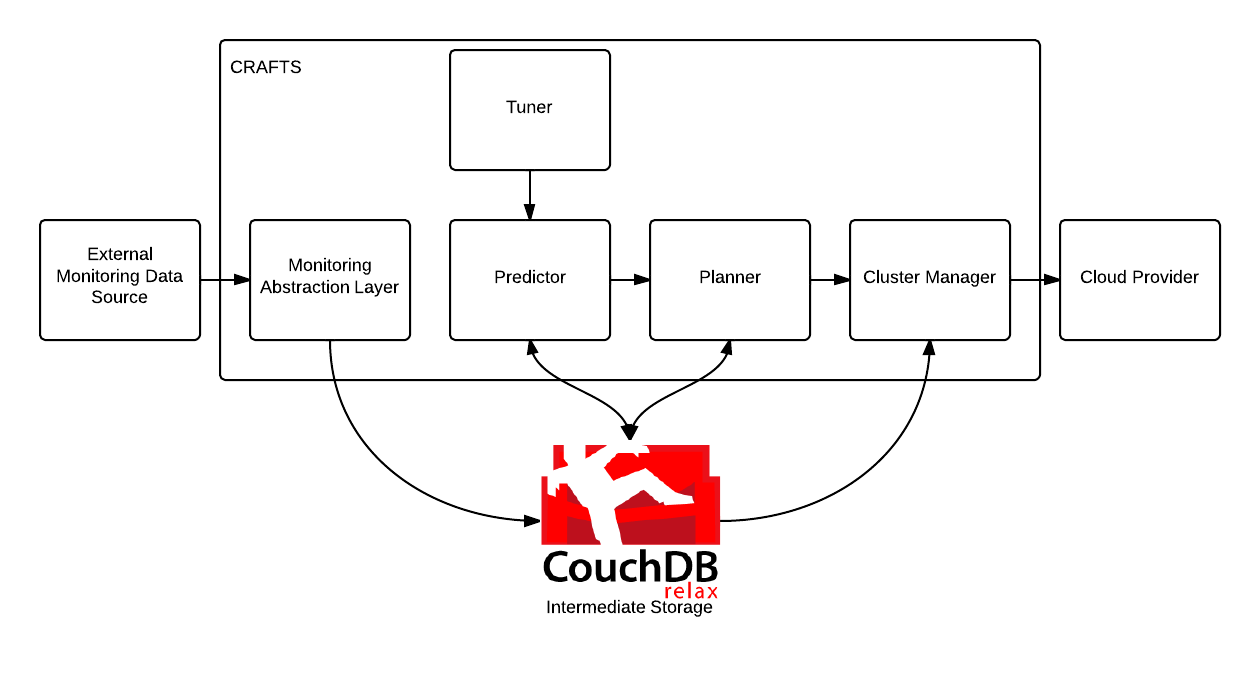
\includegraphics[width=\textwidth]{diagrams/datapipeline.png}
      \caption{Flowchart describing the CRAFTS workflow.}
      \label{fig:workflow}
\end{figure}

Data which is used for predictions is first passed in through the Monitor Abstraction Layer (\textsf{MAL}). Here, the data is put into intermediate storage for redundancy and so that aggregate calculations can be made through CouchDB's incremental MapReduce views. This data is then used by the \textsf{predictor} in order to predict future demand for the resource. These results are then also saved back to intermediate storage. Prediction data is then read by the \textsf{planner} which translates this data to a number of nodes required to maintain availability. The plan generated by the \textsf{planner} is then carried out by the \textsf{cluster manager} which makes the appropriate external API calls to acquire the cloud resources. CRAFTS also constantly tests its prediction algorithms on observed historical data and tunes prediction parameters in order to ensure the most accurate predictions possible. The rest of this chapter describes each of the data pipeline components in much greater detail.

\section{Monitor Abstraction Layer}
Data first enters the CRAFTS pipeline through the Monitoring Abstraction Layer (\textsf{MAL}). Since CRAFTS does not implement its own monitoring, the \textsf{MAL} is designed to provide a common API that allows CRAFTS to query external monitoring sources for cluster performance information. In order to mitigate load on the monitoring service, the \textsf{MAL} sends bulk requests for data at a configurable interval. This interval is called the \textbf{monitoring interval}. The data is then stored in an intermediary CouchDB database which can then be queried by CRAFTS' other components.

\section{Intermediate Storage}
Here, we describe how CRAFTS represents the monitoring data placed into intermediate storage by the \textsf{\textsf{MAL}}. This data is both inserted and stored as JSON. A diagram describing the different entities and attributes stored can be seen in \Cref{fig:datamodel}. Since CRAFTS can be implemented as a multi-tenant system, the highest level entity is that of the \textbf{tenant}. A tenant represents a single ``customer'' of CRAFTS. Data between tenants is isolated and configured independently. Tenants are implemented as CouchDB users who are given permissions to access the CRAFTS database as well as custom permissions which specify the roles they control. \textbf{Roles} are independent components of a system which are scaled independently. The primary data used by CRAFTS are samples. \textbf{Samples} are metrics collected at a given point in time. A sample document holds metrics for all the hosts assigned to the parent role at that timestamp, examples can be seen in \Cref{ap:storage}. Using CouchDB's incremental MapReduce, the sample also contains aggregates for each metric among all the hosts. These aggregates include max, min, average, count, sum, and variance. This aggregate data serves as the primary input for the \textsf{predictor}.

\begin{figure}
\centering
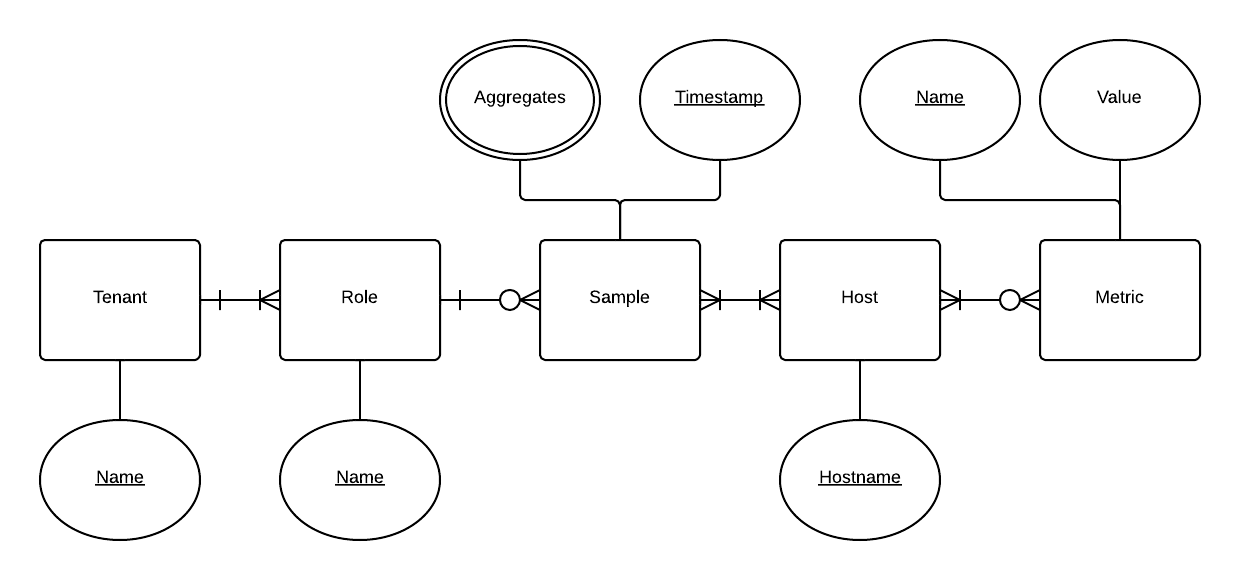
\includegraphics[width=\textwidth]{diagrams/datamodel.png}
\caption{An ER diagram describing how CRAFTS represents monitoring data.}
\label{fig:datamodel}
\end{figure}

\section{Predictor}
The purpose of the \textsf{predictor} is to determine the demand for a specific resource over the next \textbf{prediction horizon}. A prediction horizon is defined as how far into the future CRAFTS will attempt to make predictions. While which metric is predicted by the \textsf{predictor} is configurable, it typically is requests per second. Requests per second is an ideal metric because it is independent of the performance of the cluster (Netflix engineers made the same observation when building Scryer \cite{scryer}). Other useful values could include total database queries or cache requests. The \textsf{predictor} has no knowledge of the current state of the cluster, its job is solely to predict demand. The predictions generated by the \textsf{predictor} are based on a training set called the \textbf{training window}. The training window is a configurable length of time that the \textsf{predictor} may use in order to make its predictions. Details of the different prediction algorithms can be found in \Cref{ch:policies}.

Predictors may also specify configurable parameters which can be manipulated by the \textsf{tuner} in order to ensure the most accurate predictions possible. Examples of such parameters could include threshold values or offsets.

Like the \textsf{MAL}, predictors run at an interval, this interval is called the \textbf{prediction interval}. Keep in mind that the scaling interval and prediction interval are different values. A prediction interval should never be longer than the length of a prediction horizon, as this would cause there to be a period of time for which no prediction has been made. The predicted demand for the next prediction horizon is then passed to the \textsf{planner}.

\section{Planner}
The \textsf{planner} takes in the projected resource demand from the \textsf{predictor} and generates a scaling plan which is stored in the intermediate store and carried out by the \nameref{sec:clustermanager}. Generating a scaling plan involves a number of considerations that are outlined below.

\subsection{Throughput}
In order to make a translation between the predicted resource utilization and the number of nodes required to handle the demand, it is necessary for the \textsf{planner} to know the throughput of the system. To do this, the \textsf{planner} uses request and latency information acquired from the \textsf{MAL} to calculate throughput. For our purposes, we define throughput as
\begin{quote}
the maximum number of requests per second which can be served while latency is kept under a configurable value.
\end{quote}
Throughput can also be overridden manually if desired.

\subsection{VM Acquisition Time}
Since VMs will not become available the moment they are requested, it is important that the \textsf{planner} requests new nodes far enough in advance that they are operational by the time they are needed. Since this value is difficult to determine automatically, CRAFTS uses a default value of 15 minutes, but this can be overridden by the user.

\subsection{Manual Overrides}
Sometimes it is necessary to account for events which are difficult to predict. For example, holiday traffic can cause massive spikes in load, but only for a single day out of the year. This makes it difficult for CRAFTS to predict these kinds of events. Because of this, the \textsf{planner} can be overridden and a number of nodes can be specified manually to ensure that these events are handled properly, without loss to availability.

\subsection{Linear Transformation}
The \textsf{planner} assumes that the \textsf{predictor's} output is correct and makes no attempt to detect possible anomalies in the data. It does, however, add a configurable linear transformation to the prediction data. This is not done to counteract any possible error on the \textsf{predictor's} part, but instead to provide a small amount of buffer capacity in case of an anomalous spike.

\section{Cluster Manager}
\label{sec:clustermanager}
It is the \textsf{cluster manager}'s responsibility to act as a liaison between the \textsf{planner} and the cloud service which hosts the application. The \textsf{planner} will make direct calls to the \textsf{cluster manager} to schedule scaling events at certain times. The \textsf{cluster manager} must then make the appropriate calls to the host service in order to ensure that the specified number of nodes are launched at the specified time. CRAFTS also supplies a ``null'' cluster manager which will carry out no scaling actions. This can be useful when simply evaluating CRAFTS prediction methods.

\section{Tuner}
\label{sec:tuner}
It is difficult, if not impossible to assert that one prediction algorithm with one set of parameters will guarantee optimal predictions for every type of workload. For this reason, CRAFTS allows prediction algorithms to specify a set of parameters which may be tuned in order to optimize prediction accuracy. The tuner applies brute-force optimization to the \textsf{predictor}'s parameters and uses the average of the root-mean square deviation on a temporal validation as the objective function. The following sections break down and define the equations used by the tuner.

\subsection{Brute-force Optimization}
Since the predictors which we have implemented in this work have very few parameters (at most two) we have chosen to simply brute-force the parameter space rather than opting for a more elegant solution. Brute-force optimization navigates the parameter space within set bounds and samples at specified intervals. If prediction methods implemented in the future require more advanced optimizations methods, a new module can be easily swapped in.

\subsection{Temporal Validation}
Temporal validation is a technique in which a data set is partitioned into subsets where analysis is performed on one subset, the training set, and then applied to the other subset, the validation set. For the purposes of our tuning analysis, we run temporal validation using a shifting window. This window begins at the start of our known dataset, runs predictions for the next prediction horizon and then shifts forward by some interval. The resulting prediction horizons are then evaluated against the observed data using the methods outlined in the following section.

\subsection{Average of Root-mean-square Deviation}
The resulting prediction horizons are compared to the observed data using Root-mean-square deviation (RMSD). RMSD is an error measurement which takes the square root of the sum of the squared difference between the predicted and observed value divided by the sample size. The equation for RMSD can be seen in \Cref{eq:rmsd}. The RMSD is then taken for every prediction horizon. The resulting value forms the output of the objective function used in our optimization.

\begin{equation}
\label{eq:rmsd}
RSMD = \sqrt{\frac{\sum_{t=1}^n (\hat{y}_t - y_t) ^ 2}{n}}
\end{equation}